\chapter{Tinjauan Pustaka dan Dasar Teori}

\section{Tinjauan Pustaka}

Penyusunan tugas akhir ini tidak terlepas dari karya-karya tulis terdahulu yang menjadi basis ataupun inspirasi penulis dalam melaksanakan seluruh rangkaian penelitian. Subbab ini berisi ulasan dan analisis karya-karya tulis tersebut serta hubungannya dengan tugas akhir ini.

Karya tulis pertama yang dibahas adalah sebuah tesis master berjudul \textit{Through the Wormhole: Cross-OS Desktop Integration for Linux Applications} yang ditulis oleh John Ingve Olsen dan dipublikasikan pada tahun 2022 \cite{olsen-2022-through-the-wormhole}. Tesis ini merupakan karya tulis yang paling signifikan dalam penyusunan tugas akhir penulis karena memiliki topik dan tujuan yang serupa dengan tugas akhir penulis dan menjadi inspirasi terbesar dalam perancangan tugas akhir penulis. Tesis ini membahas pengintegrasian sejumlah aspek antarmuka grafis Windows Subsystem for Linux (WSL) dengan \textit{host} Windows yang dicapai melalui pengembangan sejumlah perangkat lunak pembantu:
\begin{enumerate}
    \item perangkat lunak pengelola bus sesi D-Bus (\textit{session manager}) yang menyeragamkan bus perpesanan D-Bus yang dipakai oleh sesi-sesi WSL yang berbeda dan
    \item perangkat lunak "Wormhole" itu sendiri yang mengintegrasikan aspek-aspek antarmuka grafis WSL dengan \textit{desktop} Windows.
\end{enumerate}
Olsen menggunakan bahasa pemrograman Rust dalam mengembangkan kedua perangkat lunak tersebut. Aspek-aspek yang diintegrasikan dalam tesis ini yakni
\begin{itemize}
    \item ikon status (\textit{status icons}) yang umumnya muncul di sisi kanan \textit{taskbar} pada Windows,
    \item notifikasi, dan
    \item jendela dialog pemilih berkas (\textit{file chooser}).
\end{itemize}
Meskipun Wormhole merupakan satu kesatuan perangkat lunak, Wormhole terdiri dari dua buah proses yang masing-masing berjalan di sisi \textit{host} Windows (dinamakan "\textit{backend}") dan di sisi WSL (dinamakan "\textit{bridge}"). Dalam bab kelima tesis ini, Olsen menyebutkan bahwa untuk menghubungkan proses \textit{backend} Wormhole dengan proses \textit{bridge} Wormhole, terdapat tiga pilihan metode yang mungkin dilakukan: menghubungkan dengan soket TCP/IP, berkomunikasi melalui \textit{stream} standar (\textit{standard input} dan \textit{standard output}), dan menghubungkan dengan soket Hyper-V; Olsen memilih metode ketiga karena ia merasa metode tersebut tidak memiliki kelemahan bila dibandingkan dengan kedua metode lainnya meskipun pengimplementasian metode ketiga tersebut memberikan tantangan tersendiri. Satu hal yang penulis soroti dalam tesis ini yakni mekanisme penghubungan dengan bus perpesanan D-Bus; Olsen mendesain proses \textit{bridge} agar bertindak sebagai \textit{proxy} bus perpesanan D-Bus sehingga proses \textit{backend} yang terhubung dengan proses \textit{bridge} dapat mengakses bus perpesanan D-Bus tersebut layaknya secara langsung. Secara garis besar, tesis ini memiliki perbedaan dengan tugas akhir penulis dalam tiga aspek:
\begin{itemize}
    \item cakupan fungsionalitas yang diintegrasikan (tugas akhir penulis juga mengimplementasikan sistem notifikasi, serupa dengan tesis ini, tetapi dengan tambahan fungsionalitas kontrol media),
    \item metode penghubungan (\textit{bridging}) kedua lingkungan yang digunakan (tugas akhir penulis memanfaatkan metode transportasi TCP yang tersedia pada D-Bus dengan mekanisme yang cukup berbeda dengan mekanisme yang Olsen lakukan pada tesis ini), dan
    \item perlunya pengembangan perangkat lunak pengelola sesi (\textit{session manager}) D-Bus (systemd telah didukung oleh WSL sejak September 2022 \cite{systemd-support-is-now-available-in-wsl} dan telah menjadi \textit{default} pada instalasi distribusi Ubuntu di WSL sejak perilisan Ubuntu 23.04 pada April 2023 \cite{ubuntu-2304-release-roundup-systemd-now-becomes-default-for-ubuntu-on-wsl} sehingga pengelolaan sesi bus perpesanan D-Bus saat ini telah berada di bawah kontrol systemd seperti halnya pada sistem operasi Linux asli; ketiadaan pembahasan systemd dalam tesis ini mengindikasikan bahwa waktu penulisan tesis ini terjadi sebelum hadirnya dukungan systemd tersebut sehingga diperlukan pengembangan perangkat lunak \textit{session manager} tersendiri pada saat itu).
\end{itemize}

Karya tulis kedua yang dibahas adalah sebuah tesis master berjudul \textit{Notifications in a Multi-Device Environment} yang ditulis oleh Dominik Weber dan dipublikasikan pada tahun 2015 \cite{weber2015notifications}. Secara garis besar, tesis ini membahas penanganan notifikasi antarperangkat yang memfokuskan pada aspek pengumpulan data dari pengguna. Dalam sisi teknis, tesis ini membahas pengimplementasian notifikasi multiperangkat dalam bentuk ekstensi \textit{browser} Google Chrome. Karya tulis ini memiliki sejumlah perbedaan dengan tugas akhir penulis:
\begin{itemize}
    \item Tesis ini mengimplementasikan sistem notifikasi menggunakan ekstensi \textit{browser} Google Chrome, sedangkan tugas akhir penulis mengimplementasikan sistem notifikasi dalam bentuk yang lebih \textit{native}, yakni perangkat lunak berbasis bahasa pemrograman Python.

    \item Tesis ini lebih berfokus ke aspek pengguna (dibuktikan dengan banyaknya survei yang dilakukan) dibandingkan dengan aspek teknis pengimplementasian; tugas akhir penulis lebih berfokus pada aspek pengimplementasian dan pengujian dilakukan secara mandiri oleh diri penulis sendiri.
\end{itemize}

Karya tulis ketiga yang dibahas adalah sebuah prosiding berjudul \textit{Memory forensics and the Windows Subsystem for Linux} yang dipublikasikan pada tahun 2018 \cite{lewis2018memory}. Karya tulis ini utamanya membahas pembawaan dukungan berkas-berkas \textit{executable} jenis baru, \textit{executable and linkable format} (ELF), yang umumnya berada di sistem operasi Linux ke sistem operasi Windows melalui Windows Subsystem for Linux (WSL); bersamaan dengan dukungan baru ini, terdapat peningkatan \textit{attack surface} yang, misalnya, dapat diretas oleh peretas. Karya tulis ini membahas tentang mekanisme internal WSL, berkas-berkas \textit{executable} PE (\textit{portable executable}) dan ELF (\textit{executable and linkable format}), dan forensik memori yang dilakukan terhadap aspek-aspek tersebut sehingga cukup berbeda dengan tugas akhir penulis yang membahas WSL beserta aspek-aspek integrasinya.

\section{Dasar Teori}

\subsection{Antarmuka Sistem Operasi (\textit{Shell})}

Sistem operasi tersusun atas sejumlah komponen, mulai dari komponen terdalam yang menyentuh perangkat-perangkat keras hingga komponen yang berantarmuka langsung dengan pengguna. Beberapa di antara komponen-komponen tersebut yakni \textit{kernel}, \textit{driver}, perangkat lunak sistem, \textit{shell}, dan perangkat lunak pengguna (aplikasi). Salah satu komponen yang krusial ialah \textit{shell} yang bertugas memberikan antarmuka bagi pengguna untuk dapat berinteraksi dengan sistem operasi tersebut.

Penggunaan istilah "\textit{shell}" untuk menandakan antarmuka sistem operasi pertama kali terjadi pada sekitar tahun 1964--1965 oleh Louis Pouzin ketika sedang mengembangkan sistem operasi Multics \cite{origin-of-the-shell-name}. Istilah \textit{shell} digunakan karena komponen ini adalah bagian sistem operasi terluar yang berinteraksi secara langsung dengan dunia luar dan mengelilingi komponen-komponen sistem operasi di bawahnya, sehingga dapat dianalogikan sebagai "cangkang" dari sistem operasi \cite{shell-jargon-explanation}.

Secara umum, terdapat berbagai jenis \textit{shell} yang digunakan oleh sistem-sistem operasi modern saat ini:
\begin{itemize}
    \item \textbf{\textit{Shell} berantarmuka grafis (\textit{graphical user interface})}\\
    \textit{Shell} jenis ini merupakan \textit{shell} yang paling sering pengguna temui pada zaman modern ini. Sebagian besar pengguna saat ini berinteraksi dengan perangkat komputer mereka melalui metode interaksi grafis. Antarmuka tempat pengguna berinteraksi tersebut sesungguhnya merupakan komponen \textit{shell} yang merupakan bagian dari sistem operasi pada perangkat yang bersangkutan. Sebagai contoh, \textit{shell} grafis pada sistem operasi Windows 11 terdiri atas \textit{taskbar} yang terletak di bawah layar, menu Start yang dapat dimunculkan dengan menekan tombol Start (tombol berlogo Windows di dalam \textit{taskbar}), pusat pemberitahuan/notifikasi, dan bilah pengaturan cepat (\textit{quick settings}).
    
    \item \textbf{\textit{Shell} berantarmuka baris perintah (\textit{command-line interface})}\\
    \textit{Shell} jenis ini telah ada terlebih dahulu sebelum dikembangkannya \textit{shell} berantarmuka grafis. Pada zaman modern ini, \textit{shell} berantarmuka baris perintah pun masih sering digunakan, terutama untuk kegunaan pengaksesan fungsionalitas sistem operasi tingkat lanjut, administrasi sistem, dan otomasi (\textit{scripting}). Beberapa contoh \textit{shell} berantarmuka baris perintah modern yakni PowerShell di sistem operasi Windows serta Bourne shell (\verb|sh|), Bourne-Again Shell (\verb|bash|), Z shell (\verb|zsh|), KornShell (\verb|ksh|), dan Fish shell (\verb|fish|) di sistem operasi Linux \cite{kidwai2021comparative}.
\end{itemize}

\subsection{Linux, "Mirip Unix", dan Standar POSIX}

Linux merupakan keluarga sistem operasi

\subsection{D-Bus}

D-Bus merupakan sistem komunikasi antarproses (\textit{interprocess communication}) yang populer digunakan di sebagian besar distribusi Linux. Sesuai dengan namanya, D-Bus bekerja dengan konsep arsitektur "bus" yang berarti terdapat sebuah kanal utama (bus) sebagai jalur pertukaran informasi dan terdapat sejumlah klien yang terhubung dengan kanal utama (bus) tersebut. Secara garis besar, terdapat dua komponen utama dalam penggunaan sistem D-Bus:

\begin{itemize}
    \item \textbf{\textit{Server} atau \textit{daemon} D-Bus}\\
    \textit{Server} D-Bus bertindak sebagai penyedia bus sentral tempat klien-klien D-Bus terhubung. \textit{Server} D-Bus bertugas mengelola klien-klien yang terhubung dan menyalurkan data dari sumbernya ke tujuannya dengan benar \cite{qt-introduction-to-dbus}. \textit{Server} D-Bus umumnya dijalankan oleh sebuah proses yang bernama \textit{daemon} D-Bus yang umumnya memiliki nama berkas \textit{executable} "\path{dbus-daemon}".

    \item \textbf{Klien D-Bus}\\
    Klien D-Bus merupakan istilah untuk tiap-tiap perangkat lunak yang terhubung ke bus utama D-Bus. Klien D-Bus dapat bertindak sebagai penyedia layanan (\textit{provider}) ataupun sebagai aplikasi reguler yang mengonsumsi layanan (\textit{consumer}).
\end{itemize}

\begin{figure}
    \centering
    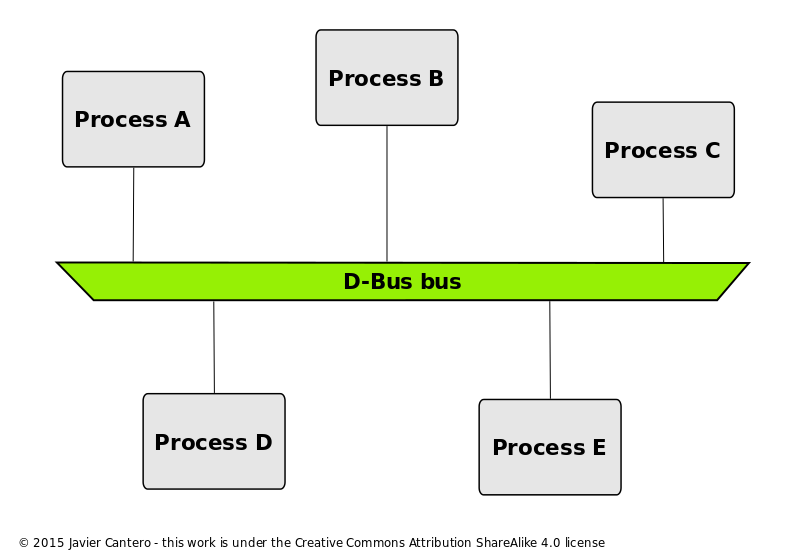
\includegraphics[width=0.75\linewidth]{archives//contents-template-pak-prapto//chapter-2/dbus-analogy-diagram.png}
    \caption{Ilustrasi bus perpesanan D-Bus \cite{dbus-bus-illustration}}
    \label{fig:enter-label}
\end{figure}

\begin{figure}
    \centering
    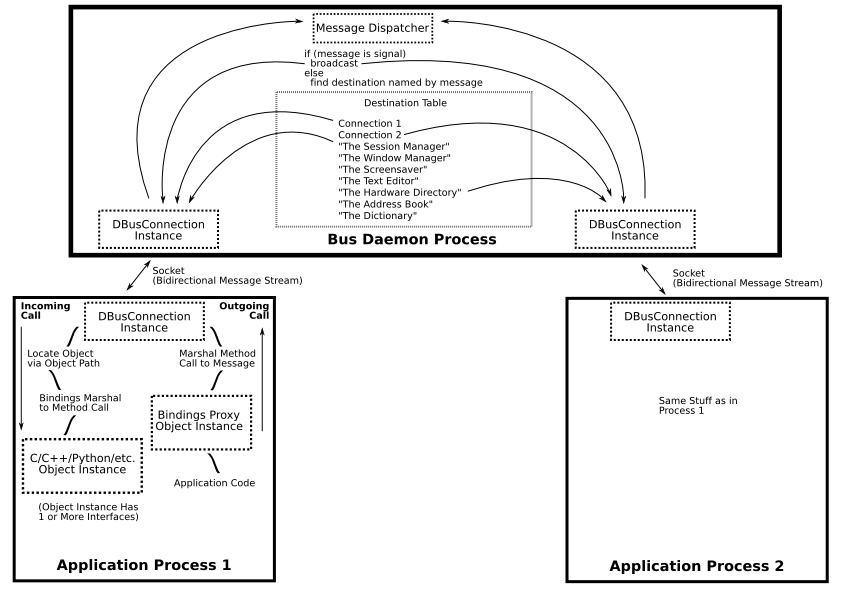
\includegraphics[width=1\linewidth]{contents//chapter-2/dbus-diagram.png}
    \caption{Diagram mendetail arsitektur D-Bus \cite{dbus-main-project-page}}
    \label{fig:enter-label}
\end{figure}

Dalam suatu sistem operasi yang sedang berjalan, dimungkinkan penjalanan lebih dari satu bus dalam satu waktu. Pada sistem operasi Linux, umumnya digunakan dua buah bus yang memiliki peran masing-masing, yaitu bus sistem (\textit{system bus}) dan bus sesi (\textit{session bus}). Bus sistem digunakan untuk mengelola dan mengadministrasi hal-hal yang bersifat penting terhadap berjalannya sistem operasi, seperti penyambungan perangkat keras baru, peringatan baterai lemah, dan status jaringan \cite{will2020trusted}. Bus sistem berjalan secara \textit{system-wide} sehingga mencakup seluruh sesi pengguna yang sedang berjalan di sistem operasi. Di sisi lain, bus sesi digunakan untuk hal-hal yang bersifat lebih mengarah ke pengguna (\textit{user-facing}) seperti pengiriman notifikasi dan sistem kontrol media, dua hal yang menjadi topik utama tugas akhir ini. Bus sesi tersedia secara lokal di tiap-tiap sesi pengguna yang sedang berjalan di suatu sistem operasi. Istilah "bus perpesanan D-Bus", "\textit{server} D-Bus", dan "\textit{daemon} D-Bus" dapat dikatakan identik dalam konteks ini; tiap-tiap bus memiliki \textit{instance} \textit{daemon} D-Bus-nya masing-masing, sehingga sistem operasi Linux secara \textit{default} memiliki dua buah \textit{instance} \textit{daemon} D-Bus yang berjalan dalam satu waktu.

Agar dapat dihubungi oleh para klien, tiap-tiap bus perpesanan D-Bus memiliki alamat yang diatur pada awal penjalanan \textit{daemon} D-Bus. Bentuk alamat yang digunakan oleh bus perpesanan D-Bus berbeda-beda sesuai dengan metode transportasi yang digunakan. Berdasarkan spesifikasi D-Bus \cite{dbus-specification}, terdapat sejumlah metode transportasi yang didukung oleh D-Bus:
\begin{itemize}
    \item \textbf{Soket Unix}\\
    Metode transportasi berbasis soket Unix menggunakan berkas soket Unix yang terletak secara lokal pada \textit{file system}. Metode transportasi ini hanya didukung apabila \textit{daemon} D-Bus berjalan di sistem operasi berbasis Unix atau mirip Unix seperti Linux dan macOS. Metode transportasi ini digunakan apabila penulisan alamat diawali oleh "\verb|unix:|".

    \item \textbf{systemd}\\
    Metode transportasi berbasis systemd memiliki konsep serupa dengan metode transportasi berbasis soket Unix, tetapi memanfaatkan sistem pengelolaan soket otomatis bernama aktivasi soket (\textit{socket activation}) yang dilakukan oleh systemd. Metode transportasi ini memanfaatkan informasi soket yang dikelola oleh systemd untuk digunakan sebagai metode transportasi D-Bus. Seperti namanya, metode transportasi ini hanya tersedia pada sistem operasi Linux yang menggunakan systemd sebagai sistem init-nya. Metode transportasi ini digunakan apabila penulisan alamat berisikan "\verb|systemd:|".
    
    \item \textbf{launchd}\\
    Metode transportasi berbasis launchd juga memiliki konsep yang serupa dengan metode transportasi berbasis soket Unix, tetapi memanfaatkan soket Unix yang telah dialokasikan oleh launchd. Mengingat sistem init launchd hanya tersedia pada sistem operasi macOS, metode transportasi ini hanya didukung apabila \textit{daemon} D-Bus berjalan di sistem operasi macOS. Metode transportasi ini digunakan apabila penulisan alamat berisikan "\verb|launchd:|".
    
    \item \textbf{TCP}\\
    Metode transportasi berbasis TCP memanfaatkan protokol TCP (Transmission Control Protocol) sebagai metode komunikasi antarklien D-Bus, baik yang terletak pada perangkat komputer yang sama maupun yang terletak pada perangkat komputer yang berbeda (\textit{remote}). Metode transportasi ini merupakan satu-satunya metode transportasi yang tersedia apabila \textit{daemon} D-Bus berjalan pada sistem operasi Windows mengingat metode-metode transportasi yang lain tidak didukung pada sistem operasi Windows. Metode transportasi ini digunakan apabila penulisan alamat diawali oleh "\verb|tcp:|" dan diikuti oleh properti-properti yang terdiri dari "\verb|host|" (wajib), "\verb|bind|" (opsional), "\verb|port|" (opsional), dan "\verb|family|" (opsional) yang penulisannya dipisahkan oleh tanda koma (misalnya "\path{tcp:localhost,port=12345,family=ipv4}").

    \item \textbf{TCP dengan metode otentikasi nonce}\\
    Metode transportasi ini identik dengan metode transportasi berbasis TCP biasa, tetapi dengan tambahan lapisan keamanan berupa otentikasi berbasis nonce. Metode otentikasi berbasis nonce memastikan bahwa hanya klien yang memiliki akses baca (\textit{read access}) pada suatu lokasi tertentu di \textit{file system} dapat terhubung ke \textit{server} D-Bus. Metode transportasi ini memiliki format penulisan alamat yang serupa dengan metode transportasi berbasis TCP biasa (sama-sama berawalan "\verb|tcp:|" dengan tambahan properti "\verb|noncefile|".

    \item \textbf{Subproses}\\
    Metode transportasi berbasis subproses bekerja dengan cara melakukan \textit{fork} pada suatu proses dan menghubungkan \textit{standard input} dan \textit{standard output} proses tersebut ke sebuah soket Unix anonim. Metode transportasi ini tidak tersedia pada sistem operasi Windows. Metode transportasi ini digunakan apabila alamat diawali oleh "\verb|unixexec:|".
\end{itemize}

Seperti yang telah disebutkan pada tiap-tiap deskripsi metode transportasi di atas, metode transportasi ditentukan secara otomatis sesuai dengan format penulisan alamat bus perpesanan D-Bus yang telah diatur. Alamat bus perpesanan D-Bus dapat diatur melalui dua tempat: argumen penjalanan \textit{daemon} D-Bus dan berkas konfigurasi. Metode pengaturan alamat bus perpesanan D-Bus melalui argumen penjalanan \textit{daemon} D-Bus dilakukan dengan menambahkan argumen berbentuk \lstinline[language=bash,columns=fixed]{--address="<tuliskan alamat yang diinginkan di sini>"}. Metode pengaturan alamat melalui argumen akan menimpa (\textit{override}) pengaturan apa pun yang dilakukan di berkas konfigurasi. Di sisi lain, metode pengaturan alamat bus perpesanan D-Bus melalui berkas konfigurasi dilakukan dengan cara memodifikasi berkas konfigurasi \textit{default} yang telah ada (berkas konfigurasi \textit{default} bus sistem berada di \path{/usr/share/dbus-1/system.conf} dan berkas konfigurasi \textit{default} bus sesi berada di \path{/usr/share/dbus-1/session.conf}) atau membuat berkas konfigurasi baru berekstensi berkas "\verb|.conf|" dan memuatnya pada saat penjalanan \textit{daemon} D-Bus melalui argumen \lstinline[language=bash,columns=fixed]{--config-file=<lokasi berkas konfigurasi>}.

Dalam mengidentifikasi dirinya sendiri dan berkomunikasi dengan klien lain, tiap-tiap klien yang terhubung dengan bus perpesanan D-Bus mengemban sejumlah elemen yang didesain agar memiliki kemiripan dengan konsep-konsep pemrograman berorientasi objek yang telah familier bagi banyak orang. Berikut elemen-elemen yang dimaksud.
\begin{itemize}
    \item \textbf{Nama bus (\textit{bus name})}\\
    Tiap-tiap klien D-Bus memiliki identitas berupa "nama bus" yang digunakan untuk mengidentifikasi klien tersebut dalam suatu bus perpesanan D-Bus. Nama bus terdiri dari dua jenis, nama bus unik (\textit{unique name}) dan nama bus yang dikenal (\textit{well-known name}), dan tiap-tiap klien dapat memiliki lebih dari satu nama bus. Secara \textit{default}, tiap-tiap klien baru yang terhubung ke suatu bus perpesanan D-Bus akan mendapatkan nama bus unik (diberikan secara otomatis oleh \textit{daemon} D-Bus) yang tersusun atas sejumlah angka yang dimulai oleh tanda titik dua (misalnya "\verb|:34-907|"). Perlu diingat bahwa istilah "nama bus" di sini berarti nama masing-masing klien yang terhubung dalam suatu bus perpesanan, bukan nama bus perpesanan itu sendiri \cite{official-introduction-to-dbus}.
    \item \textbf{Objek (\textit{object})}\\
    Objek dalam konteks komunikasi D-Bus merupakan ujung-ujung komunikasi (\textit{endpoint}) yang dimiliki oleh klien di dalam suatu bus perpesanan D-Bus. Tiap-tiap klien D-Bus dapat memiliki lebih dari satu objek.
    \item \textbf{Antarmuka (\textit{interface})}\\
    Antarmuka dalam konteks komunikasi D-Bus merupakan suatu "kontrak" yang disetujui oleh berbagai klien yang digunakan untuk memfasilitasi komunikasi antarklien. Antarmuka diperlukan agar dua klien dapat berkomunikasi dengan bentuk dan struktur data yang sama yang telah disetujui oleh masing-masing pihak.
\end{itemize}

Secara garis besar, proses komunikasi di dalam suatu bus perpesanan D-Bus dilakukan dalam bentuk "pesan" (\textit{message}). Pesan-pesan dalam D-Bus dapat dikategorikan menjadi dua jenis di bawah ini yang juga memiliki kemiripan dengan konsep pemrograman berorientasi objek.
\begin{itemize}
    \item \textbf{Metode (\textit{method})}\\
    Metode merupakan pesan yang dikirimkan secara spesifik dan terarah dari klien pengirim (\textit{sender}) ke tujuan (\textit{destination}) yang jelas. Pesan jenis metode dikirimkan dengan cara memanggil metode yang bersangkutan pada objek D-Bus yang diinginkan.
    \item \textbf{Sinyal (\textit{signal})}\\
    Sinyal merupakan pesan yang dikirimkan secara tidak terarah (tidak memiliki tujuan spesifik). Pesan berjenis sinyal disebarluaskan (\textit{advertise}) di dalam bus perpesanan untuk didengarkan oleh klien-klien lain yang berkepentingan.
\end{itemize}

Selain dua jenis pesan di atas, objek-objek pada klien D-Bus juga memiliki elemen bernama "properti" (\textit{property}) yang juga berkonsep serupa dengan pemrograman berorientasi objek. Properti pada suatu objek D-Bus umumnya berisi informasi-informasi yang berkaitan dengan objek tersebut dan/atau klien yang memiliki objek tersebut. Pada umumnya, setiap pergantian nilai properti akan menyebabkan sinyal bernama "\path{PropertiesChanged}" pada antarmuka "\path{org.freedesktop.DBus.Properties}" tersebar sehingga pergantian nilai properti tersebut dapat diketahui oleh klien-klien lain yang berkepentingan.

Dalam menginspeksi bus perpesanan D-Bus, terdapat berbagai macam perangkat lunak atau peralatan (\textit{tools}) yang dapat membantu. Secara \textit{default}, perangkat lunak D-Bus yang terinstal juga memiliki peralatan-peralatan bawaan seperti \verb|dbus-monitor| dan \verb|dbus-send| yang dapat bermanfaat untuk memeriksa serta berinteraksi langsung dengan bus perpesanan D-Bus dalam antarmuka baris perintah (\textit{command-line interface}). Selain itu, tersedia pula solusi-solusi pihak ketiga seperti perangkat lunak D-Feet yang dapat memeriksa bus perpesanan D-Bus dalam antarmuka grafis (\textit{graphical user interface}).

\begin{figure}[h]
    \centering
    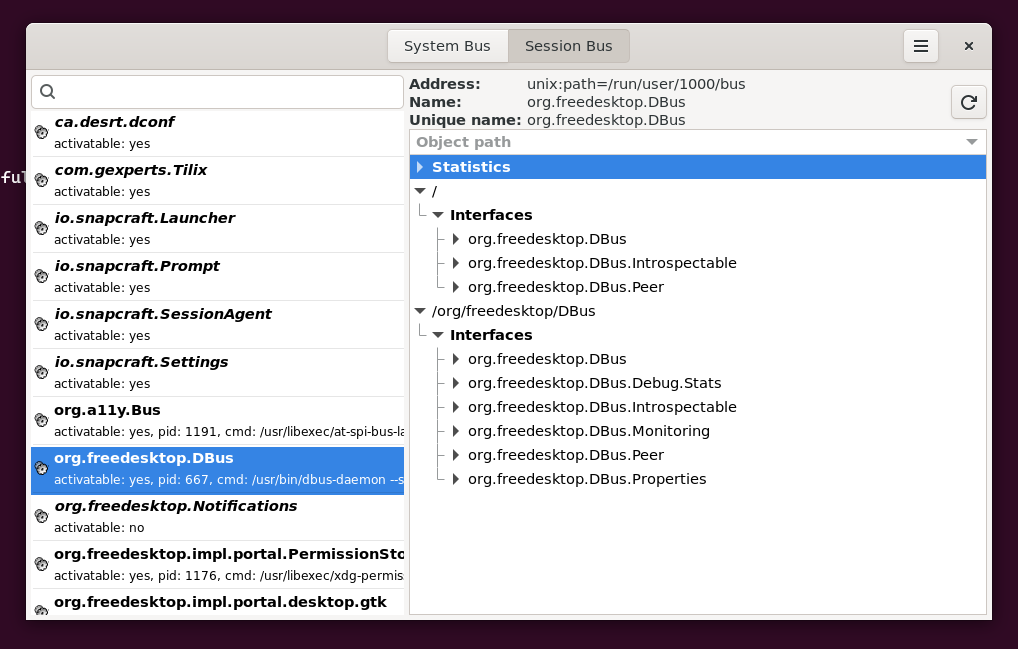
\includegraphics[width=0.75\linewidth]{archives//contents-template-pak-prapto//chapter-2/dfeet-window-screenshot.png}
    \caption{Tangkapan layar perangkat lunak "D-Feet" yang berjalan di Windows Subsystem for Linux (WSL)}
    \label{fig:enter-label}
\end{figure}

% \subsection{Sistem Init systemd}

% systemd merupakan salah satu sistem init yang tersedia untuk digunakan di sistem operasi Linux di samping sistem-sistem init lain seperti SysV Init, .

\subsection{Windows Subsystem for Linux (WSL)}

Windows Subsystem for Linux merupakan usaha Microsoft dalam membawa kompatibilitas Unix/Linux ke dalam lingkungan Windows. Secara garis besar, terdapat dua versi WSL yang telah dirilis dengan konsep dan arsitektur yang berbeda.
\begin{itemize}
    \item \textbf{Windows Subsystem for Linux versi 1 (WSL1)}
    WSL1 memanfaatkan sebuah lapisan penerjemah panggilan-panggilan sistem (\textit{syscalls}) yang dipanggil oleh perangkat-perangkat lunak Linux agar diterjemahkan menjadi panggilan-pangiglan sistem (\textit{syscalls}) ekuivalen yang terdapat di Windows. WSL1 adalah varian WSL yang diluncurkan pada pengenalan WSL pertama kali di Windows 10 pada tahun 2016.

    \item \textbf{Windows Subsystem for Linux versi 2 (WSL2)}
    WSL2 memanfaatkan sebuah \textit{virtual machine} Hyper-V dengan sejumlah integrasi lebih lanjut agar tidak terasa seperti penjalanan \textit{virtual machine} tradisional. WSL2 menjalankan \textit{kernel} Linux asli yang tervirtualisasi sehingga meningkatkan cakupan dukungan perangkat lunak Linux dibandingkan dengan WSL1.
\end{itemize}

% Pada perheletan pengembang tahunan Microsoft Build 2021, Microsoft menyatakan bahwa mereka akan mendukung 

Pada tahun 2021, Microsoft merilis sistem operasi Windows 11 yang membawa sejumlah perkembangan; salah satu perkembangan tersebut terdapat pada WSL. Windows 11 mendukung penjalanan perangkat lunak Linux berantarmuka grafis (GUI) secara langsung. Microsoft menamakan fitur baru ini "Windows Subsystem for Linux GUI (WSLg)".

\begin{figure}
    \centering
    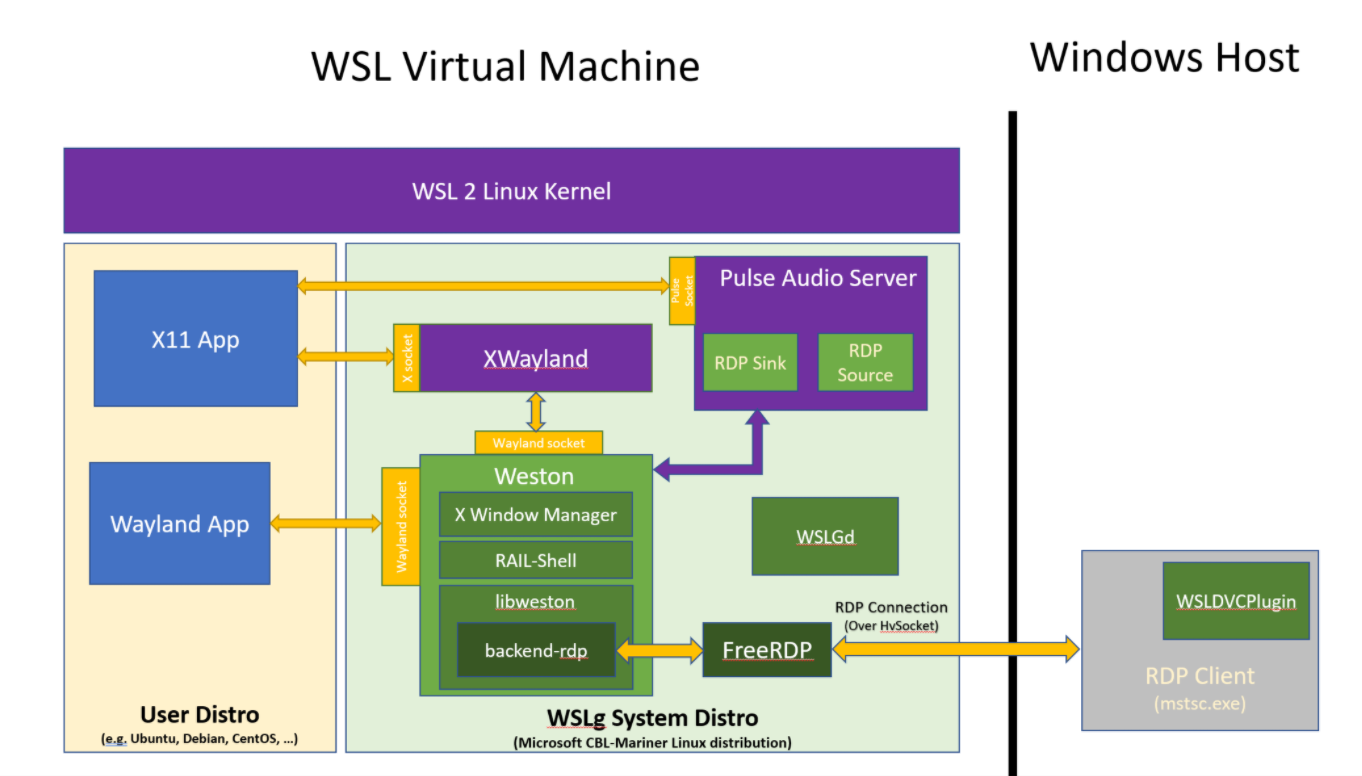
\includegraphics[width=0.5\linewidth]{wslg-architecture.png}
    \caption{Arsitektur Windows Subsystem for Linux GUI (WSLg \cite{wslg-architecture})}
\end{figure}

% https://link.springer.com/chapter/10.1007/978-1-4842-6873-5_1

\section{Analisis Perbandingan Metode}

Dalam penyusunan tugas akhir ini, penulis mengkaji serta membandingkan metode-metode yang mungkin dilakukan untuk sejumlah aspek pengerjaan. Aspek-aspek yang dimaksud yaitu penghubungan (\textit{bridging}) lingkungan Windows Subsystem for Linux (WSL) dengan lingkungan \textit{host} Windows dan penentuan bahasa dan platform pemrograman yang paling praktis dan cocok digunakan dalam pengembangan perangkat lunak yang terlibat.

Dalam aspek penghubungan lingkungan Windows Subsystem for Linux (WSL) dengan lingkungan \textit{host} Windows, metode yang dipilih menentukan jumlah dan cakupan perangkat lunak yang perlu dikembangkan, tingkat kesulitan pengembangan perangkat lunak tersebut, serta efisiensi penjalanan perangkat lunak yang telah jadi. Berikut pemaparan empat metode yang mungkin dilakukan.
\begin{enumerate}
    \item Lingkungan WSL dihubungkan dengan lingkungan \textit{host} Windows melalui \textit{socket} Unix. Hal ini dimungkinkan dengan diperkenalkannya dukungan \textit{socket} Unix (AF\_UNIX) pada sistem operasi Windows 10 ke atas pada tahun 2017 \cite{bringing-afunix-to-windows}. Namun, penelusuran lebih lanjut mengindikasikan bahwa kemampuan ini rupanya hanya mendukung Windows Subsystem for Linux versi 1 (WSL1) dan belum mendukung Windows Subsystem for Linux versi 2 (WSL2) \cite{github-issues-afunix-not-supported-in-wsl2}. Oleh karena itu, mengingat kemampuan grafis (\textit{graphical user interface}) pada Windows Subsystem for Linux hanya tersedia pada Windows Subsytem for Linux versi 2 (WSL2), metode ini tidak relevan dengan tujuan skripsi ini.
    
    \item Lingkungan WSL dihubungkan dengan lingkungan \textit{host} Windows dengan memanfaatkan \textit{server} HTTP. Metode ini ikut dipertimbangkan mengingat pengalaman penulis yang cukup banyak berhubungan dengan bidang pengembangan web (\textit{web development}). Metode ini dapat dibagi kembali menjadi dua submetode:
    
    \begin{enumerate}
        \item Penghubungan kedua lingkungan melibatkan dua buah \textit{server} HTTP yang masing-masing berjalan di sisi WSL dan di sisi \textit{host} Windows. Dua buah \textit{server} diperlukan karena komunikasi bersifat dua arah: WSL mengirimkan konten yang ingin ditampilkan ke sisi \textit{host} Windows dan \textit{host} Windows mengomunikasikan hasil interaksi pengguna (\textit{user input}) kembali ke sisi WSL. Meskipun implementasi submetode ini dapat dibuat seefisien mungkin, penjalanan dua buah \textit{server} tetap saja terasa kurang efisien, terutama bila dibandingkan dengan metode-metode lainnya.
        
        \item Penghubungan kedua lingkungan menggunakan cukup satu buah \textit{server} saja untuk menghindari duplikasi penggunaan \textit{resources}, tetapi memanfaatkan teknologi yang memungkinkan komunikasi secara dua arah seperti HTTP \textit{long polling} dan WebSocket. Penggunaan HTTP \textit{long polling} memiliki kemungkinan menghasilkan performa yang kurang efisien \cite{problems-in-http-long-polling}, sedangkan penggunaan WebSocket sama saja dengan penggunaan Unix \textit{socket} biasa namun dengan \textit{overhead} protokol HTTP yang dapat berefek pada performa.
    \end{enumerate}
    
    \item Lingkungan WSL dihubungkan dengan lingkungan \textit{host} Windows dengan komunikasi secara tekstual atau terserialisasi (\textit{serialized}). Pertukaran informasi berbentuk teks (tekstual) ini dapat melalui berbagai perantara; berikut beberapa di antaranya.
    \begin{enumerate}
        \item Informasi tekstual dipertukarkan melalui berkas \textit{executable} pembantu (\textit{helper}) sebagai argumen pengeksekusian berkas \textit{executable} tersebut. Ditentukan dua buah berkas \textit{executable} yang masing-masing bertugas mengirimkan informasi ke sisi \textit{host} Windows dan mengirimkan informasi ke sisi WSL. Pada sisi WSL, hal ini dimungkinkan oleh kemampuan WSL menjalankan berkas \textit{executable} Windows (umumnya berekstensi \verb|.exe|) secara langsung di dalam \textit{command-line} WSL \cite{msdocs-run-windows-tools-from-linux}. Pada sisi Windows, hal ini dimungkinkan oleh kemampuan memanggil WSL secara programatik atau \textit{scripted} dengan perintah yang telah ditetapkan. Sebagai contoh, pengiriman informasi dari sisi WSL dapat dilakukan dengan perintah
        \begin{lstlisting}[language=bash]
# Di shell bash
/path/to/fwsl-send-to-windows.exe --data="<insert JSON-serialized data here>"\end{lstlisting}
        dan pengiriman informasi dari sisi Windows ke sisi WSL dapat dilakukan dengan perintah
        \begin{lstlisting}
# Di shell PowerShell atau cmd.exe
wsl.exe /path/to/fwsl-send-to-wsl --data="<insert JSON-serialized data here>"\end{lstlisting}

        \item Informasi tekstual dipertukarkan melalui mekanisme \textit{piping}. Cara pertukaran data ini serupa dengan penggunaan berkas \textit{executable} pembantu (\textit{helper}) pada submetode (a), namun data disalurkan melalui \textit{standard stream} (seperti \textit{standard input} dan \textit{standard output}) dan dihubungkan dengan \textit{pipe} alih-alih diletakkan sebagai argumen suatu berkas \textit{executable}. Pertukaran data dengan cara ini tetap memerlukan berkas-berkas \textit{executable} sebagai pengirim dan/atau penerima data. Tetapi, berbeda dengan submetode (a), submetode ini memungkinkan penggunaan perangkat lunak utama itu sendiri sebagai pengirim dan penerima data. Pertukaran data difasilitasi oleh berkas \textit{named pipe} sebanyak dua buah yang masing-masing menangani pengiriman data ke tiap-tiap arah (menuju Windows dan menuju WSL).
        \begin{verbatim}
 ________________               ________________
|                |             |                |
|           StdIn(== ← === ← ==(StdOut          |
|    Windows     |             |   WSL bridge   |
|    bridge      |             |                |
|          StdOut)== → === → ==)StdIn           |
|________________|             |________________|

        \end{verbatim}

        \item Informasi tekstual dipertukarkan dengan memanfaatkan perintah \verb|dbus-send| dan \verb|dbus-monitor| secara programatik. Mengingat topik utama skripsi ini selalu berkaitan dengan protokol D-Bus, submetode ini dapat mensimplifikasi rangkaian proses pengerjaan karena menggunakan peralatan yang berasal dari D-Bus itu sendiri. Sebagai contoh, dengan pemantauan keluaran (\textit{output}) perintah \verb|dbus-monitor|, pemulaian pemutaran media (musik, video, dan lain-lain) dari suatu perangkat lunak yang berjalan di dalam WSL menghasilkan keluaran
        \begin{lstlisting}
signal time=1702386858.242218 sender=:1.19 -> destination=(null destination) serial=24 path=/org/mpris/MediaPlayer2; interface=org.freedesktop.DBus.Properties; member=PropertiesChanged
   string "org.mpris.MediaPlayer2.Player"
   array [
      dict entry(
         string "PlaybackStatus"
         variant             string "Playing"
      )
   ]
   array [
   ]\end{lstlisting}
        dan apabila pemutaran media tersebut ingin dijeda (\textit{pause}), dapat dijalankan perintah berikut
        \begin{lstlisting}[language=bash]
dbus-send --dest=org.mpris.MediaPlayer2.spotify /org/mpris/MediaPlayer2 org.mpris.MediaPlayer2.Player.PlayPause\end{lstlisting}
        Meskipun demikian, proses integrasi dalam skripsi ini melibatkan lebih dari sekadar perintah-perintah D-Bus dan dapat dipastikan membutuhkan perangkat lunak tambahan. Sebagai contoh, sejumlah fungsi yang dilayani melalui D-Bus seperti penanganan notifikasi memerlukan layanan (\textit{service}) yang diregistrasikan secara eksplisit di bus perpesanan D-Bus yang bersangkutan; submetode ini hanya mengandalkan metode yang serupa dengan "\textit{sniffing}" dan tidak benar-benar memiliki identitas dan keberadaan yang teregistrasi sehingga fungsi penanganan notifikasi tetap tidak akan bisa bekerja. Oleh karena itu, akan lebih baik apabila seluruh fungsionalitas dan logika dalam pengerjaan skripsi ini disatukan ke dalam perangkat lunak tambahan tersebut. Selain itu, keluaran (\textit{output}) perintah \verb|dbus-monitor| tidak selalu lengkap (pada contoh keluaran perintah \verb|dbus-monitor| di atas, tidak ada informasi bahwa perangkat lunak Spotify adalah perangkat lunak yang memulai memainkan media), sehingga submetode ini kurang bisa diandalkan.
    \end{enumerate}
    
    \item Lingkungan Windows Subsystem for Linux (WSL) dihubungkan dengan lingkungan \textit{host} Windows dengan meng-\textit{extend} jangkauan bus perpesanan D-Bus hingga dapat diakses secara langsung di dalam lingkungan Windows, sehingga perangkat lunak di Windows dapat langsung menghubungi bus perpesanan D-Bus yang berjalan di WSL. Hal ini dicapai dengan cara mengatur konfigurasi \verb|dbus-daemon| di WSL agar dapat diakses melalui TCP (di samping konfigurasi soket Unix \textit{default} yang telah ada) dan mengonsumsi alamat TCP yang ditentukan di perangkat lunak \textit{bridge} yang berjalan di Windows. Metode ini memiliki keuntungan tersendiri: mengingat koneksi bus perpesanan D-Bus saat ini tersedia secara langsung di lingkungan Windows, penyediaan \textit{notification server} dan \textit{MPRIS server} dapat dilakukan secara langsung oleh perangkat lunak \textit{bridge} di sisi Windows, sehingga menghilangkan kebutuhan penjalanan perangkat lunak \textit{bridge} kedua di lingkungan WSL.
\end{enumerate}

Berdasarkan penjabaran dan analisis perbandingan metode penghubungan lingkungan WSL dengan lingkungan \textit{host} Windows, dipilih metode keempat mengingat metode penghubungannya yang cukup \textit{straightforward} dan penggunaan protokol TCP yang relatif lebih efisien dibandingkan dengan metode-metode lainnya.

Dalam aspek bahasa dan platform pemrograman, dipertimbangkan berbagai hal seperti kelengkapan integrasi dengan \textit{application programming interface} (API) \textit{shell} Windows dan kemampuan berkomunikasi dengan D-Bus (baik dengan solusi bawaan atau pihak pertama, apabila tersedia, maupun dengan bantuan pustaka pihak ketiga yang tersedia pada bahasa pemrograman tersebut). Berikut perbandingan platform dan bahasa pemrograman yang dapat digunakan yang disajikan dalam bentuk tabel.

\begin{table}[h]
    \centering
    \caption{Perbandingan platform dan bahasa pemrograman}
    \begin{tabularx}{\textwidth}{|l|X|X|} \hline
        \textbf{Platform} & \textbf{Integrasi \textit{Shell} Windows} & \textbf{Integrasi D-Bus}\\ \hline
        C\# & Tersedia (mengingat C\# adalah salah satu platform \textit{native} di Windows & Terbatas dan kurang terdokumentasi (\textit{undocumented})\\ \hline
        Python & Tersedia melalui \textit{binding} pihak ketiga & Tersedia pustaka-pustaka (\textit{library}) yang beraneka ragam\\ \hline
    \end{tabularx}
\end{table}

Meskipun bahasa pemrograman C\# didukung secara lebih baik oleh sistem operasi Windows, ketiadaan dukungan integrasi dengan D-Bus yang memungkinkan menghalangi penggunaan bahasa pemrograman C\# sebagai opsi yang \textit{viable}. Oleh karena itu, dipilih bahasa penggunaan Python yang memiliki dukungan lebih baik dalam penghubungan dengan D-Bus meskipun harus menggunakan \textit{binding} tambahan untuk mengakses beragam API yang terdapat di Windows.

\section{Pertanyaan Tugas Akhir}

Dalam serangkaian pengerjaan tugas akhir ini, penulis menemukan beberapa pertanyaan yang berkaitan dengan metode yang telah dipilih. Pertanyaan-pertanyaan ini perlu dijawab sebelum dapat melanjutkan ke langkah selanjutnya dalam pengerjaan.

\begin{enumerate}
    \item Perangkat lunak \verb|dbus-daemon| dapat melakukan \textit{listening} ke lebih dari satu alamat apabila telah diatur pada berkas konfigurasi (misalnya pada berkas \path{/usr/share/dbus-1/session.conf} untuk bus \textit{session}). Namun, \verb|dbus-daemon| juga memiliki seperangkat argumen eksekusi \cite{dbus-daemon-man-page} yang beberapa di antaranya dapat menimpa (\textit{override}) konfigurasi yang telah dilakukan pada berkas konfigurasi; salah satu argumen yang menarik perhatian yaitu argumen \verb|--address|. Apakah argumen ini mendukung pemberian lebih dari satu alamat? Apabila argumen ini hanya mendukung satu alamat, apa yang terjadi jika argumen ini digunakan dalam pemanggilan \verb|dbus-daemon| saat konfigurasi yang tertimpa (\textit{override}) pada berkas konfigurasi memuat lebih dari satu alamat? Apakah penggunaan argumen ini hanya menimpa (\textit{override}) satu buah alamat pada berkas konfigurasi saja atau menimpa (\textit{override}) semua alamat yang telah diatur pada berkas konfigurasi?

    % \item Selain berkomunikasi secara lokal melalui \textit{socket} Unix, D-Bus juga memiliki kemampuan melalui protokol TCP, sehingga memungkinkan komunikasi dengan klien-klien yang berjalan di lingkungan di luar sistem operasi saat ini, baik di perangkat komputer lain (penghubungan secara \textit{remote}) maupun di sebuah \textit{virtual machine} pada perangkat komputer fisik yang sama. Apakah komputer lain tersebut memerlukan penjalanan \verb|dbus-daemon| milik komputer itu sendiri atau perangkat lunak \textit{client} di komputer tersebut dapat langsung terhubung ke D-Bus pusat tanpa memerlukan adanya \verb|dbus-daemon| tambahan yang berjalan pada komputer tersebut? (TODO: Rephrase this one.)
\end{enumerate}
